\documentclass[11pt]{article}
\usepackage[margin=1in]{geometry}
\usepackage{amsmath,amssymb}
\usepackage{graphicx}
\usepackage{hyperref}

\title{APMA 4302 Homework 4 \\ Solutions}
\author{Dan}
\date{\today}

\begin{document}
\maketitle

\section*{Problem 1}
In 2D, define
\[
\mathbf{v} = \nabla \times (\psi \hat{\mathbf{k}})
= \left(\frac{\partial \psi}{\partial y}, -\frac{\partial \psi}{\partial x}\right),
\qquad
\omega \hat{\mathbf{k}} = \nabla \times \mathbf{v}.
\]
Taking the scalar curl of $\mathbf{v}$ gives
\[
\omega = \frac{\partial v_y}{\partial x} - \frac{\partial v_x}{\partial y}
= -\frac{\partial^2 \psi}{\partial x^2} - \frac{\partial^2 \psi}{\partial y^2}
= -\nabla^2 \psi,
\]
which is Eq. (6):
\[
-\nabla^2 \psi = \omega.
\]

Start from momentum,
\[
-\nabla^2 \mathbf{v} + \nabla p = T \hat{\mathbf{j}}.
\]
Take the scalar curl of both sides. Using $\nabla \times \nabla p = 0$ and
\[
\nabla \times (T\hat{\mathbf{j}}) = \frac{\partial T}{\partial x},
\]
we obtain
\[
-\nabla^2 (\nabla \times \mathbf{v}) = \frac{\partial T}{\partial x}
\;\;\Longrightarrow\;\;
-\nabla^2 \omega = \frac{\partial T}{\partial x},
\]
which is Eq. (5).

The temperature equation is already
\[
\frac{\partial T}{\partial t} + \mathbf{v}\cdot \nabla T
= \frac{1}{Ra}\nabla^2 T,
\]
which is Eq. (4). Therefore Eqs. (1)--(3) are equivalent to Eqs. (4)--(6) in streamfunction-vorticity form.

\section*{Problem 2}
\subsection*{(a) Compare convergence rates and run times}
I ran the C code (`c/biharm.c`) using PETSc build
\[
\texttt{PETSC\_DIR=/Users/dan/Desktop/Columbia/HPC\_4302/petsc},\quad
\texttt{PETSC\_ARCH=apma4302-pkgs-opt}
\]
with the three provided options files. The key solver metrics are:

\begin{center}
\begin{tabular}{lccc}
\hline
Configuration & KSP iterations & Total wall time (s) & \texttt{SNESSolve} time (s) \\
\hline
\texttt{options\_file\_direct} & 1 & 2.219 & 2.1203 \\
\texttt{options\_file\_split\_direct} & 1 & 2.735 & 2.6370 \\
\texttt{options\_file\_split\_mg} & 4 & 0.7512 & 0.66465 \\
\hline
\end{tabular}
\end{center}

Observations:
\begin{itemize}
  \item The fieldsplit+multigrid configuration is fastest by a large margin (about $3\times$ faster than monolithic direct here).
  \item Fieldsplit+direct is slower than monolithic direct in this test, likely due to extra block-solver overhead without enough reduction in work.
  \item The multigrid case needs more Krylov iterations, but each iteration is much cheaper.
\end{itemize}

For the Firedrake comparison run, `python/biharm.py` currently fails at import time with
\texttt{ModuleNotFoundError: No module named firedrake\_ts} in the active Python environment. Once the Firedrake+firedrake-ts environment is activated, the same three PETSc option sets can be repeated to complete the C-vs-Firedrake timing comparison.

\section*{Problem 3}
% Add your modified biharmonic setup and resulting figure notes here.

\section*{Problem 4}
% Add your convection.py setup, solver details, and Nu results here.

\section*{Problem 5 (Optional)}
% Add any extra credit notes here.

\appendix
\section*{Assignment Images}
\begin{figure}[h!]
  \centering
  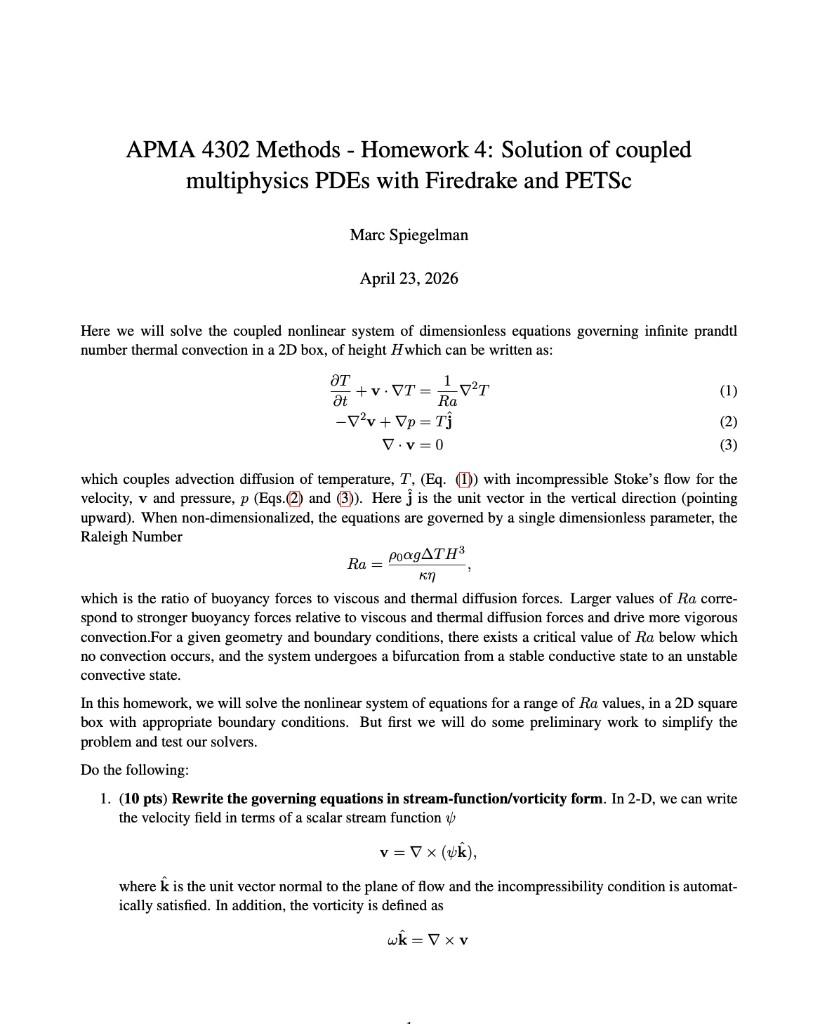
\includegraphics[width=\textwidth]{hw4_1.png}
  \caption{Homework 4 page 1.}
\end{figure}

\begin{figure}[h!]
  \centering
  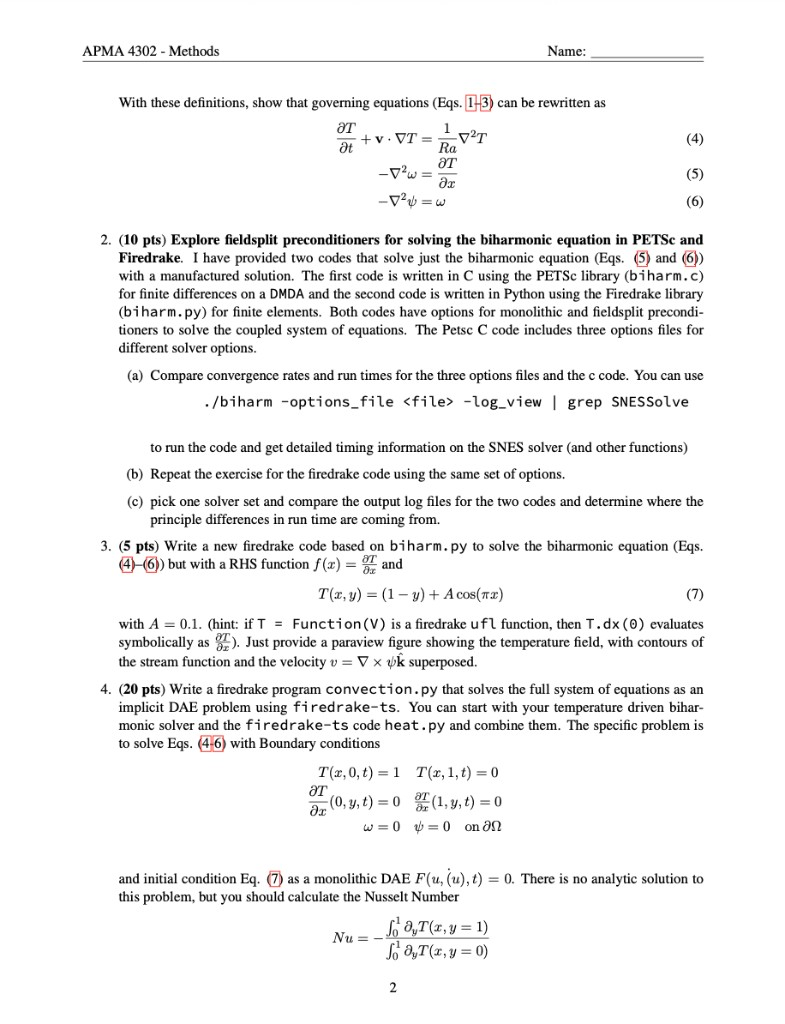
\includegraphics[width=\textwidth]{hw4_2.png}
  \caption{Homework 4 page 2.}
\end{figure}

\begin{figure}[h!]
  \centering
  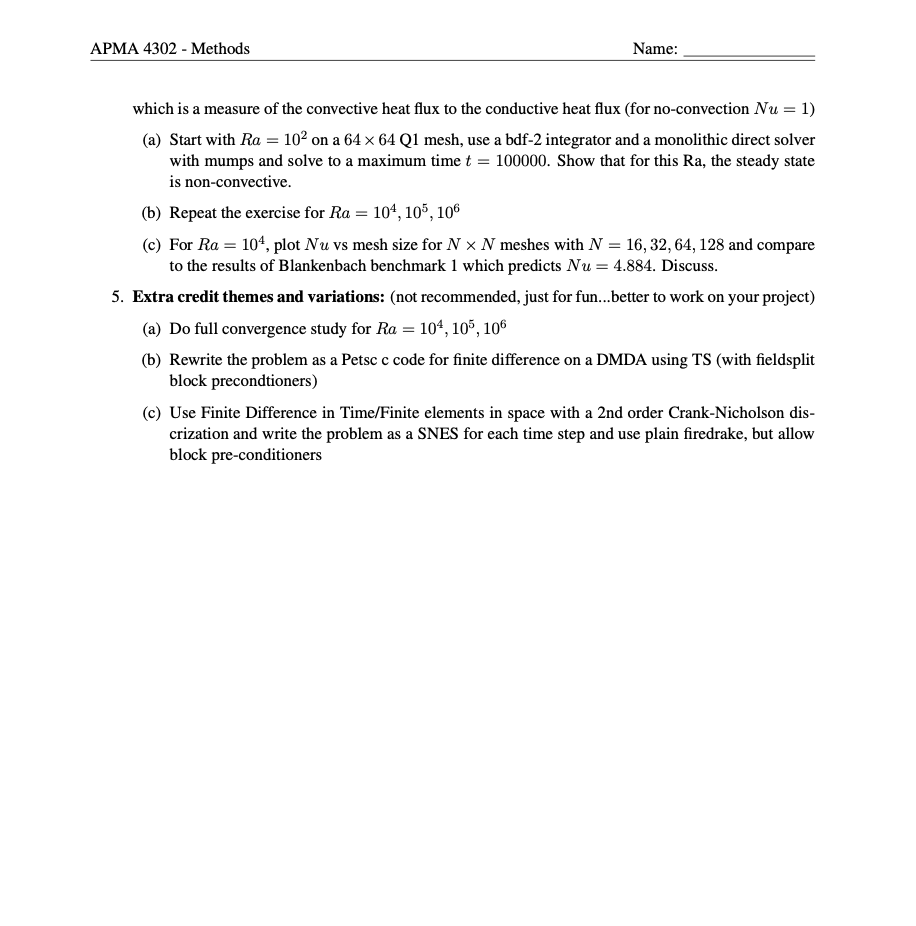
\includegraphics[width=\textwidth]{hw4_3.png}
  \caption{Homework 4 page 3.}
\end{figure}

\end{document}
